\documentclass[conference]{IEEEtran}
\IEEEoverridecommandlockouts
\usepackage[T1]{fontenc}
\usepackage{cite}
\usepackage{amsmath,amssymb,amsfonts}
\usepackage{algorithmic}
\usepackage{graphicx}
\usepackage{textcomp}
\usepackage{xcolor}
\usepackage{booktabs}
\usepackage{multirow}
\usepackage{siunitx}
\usepackage{url}

\begin{document}

\title{Adaptive Active Noise Cancellation for Hearables using Interacting Multiple Model (IMM) Filters}

\author{%
\IEEEauthorblockN{Muhammed Ali Yesin, Mehmet Akif Takcı}
\IEEEauthorblockA{\textit{Dept.\ of Electrical and Electronics Engineering} \\
\textit{Marmara University}\\
Istanbul, T\"urkiye \\
EE4084: Kalman and Bayesian Filters, Spring 2026}
}

\maketitle

\begin{abstract}
Active Noise Cancellation (ANC) for hearable devices is a problem of switching
regimes. A wearer crosses several acoustic environments within minutes, a quiet
office, broadband traffic, modulated speech babble, and impulsive wind, and each
one calls for a different operating point on the trade-off between convergence and
misalignment of an adaptive controller. Classical Normalized Least Mean Squares
(NLMS) and single mode Kalman filters are governed by one step size or one process
noise variance, so they cannot be optimal across every regime at once. We develop
an Interacting Multiple Model Kalman Filter (IMM-KF), running at the sample rate,
whose state is the weight vector of the adaptive FIR controller and whose bank of
four Kalman filters, one conditioned on each mode, is combined through the usual
cycle of mixing, filtering, update, and combination. Because the observation in the
Filtered-$x$ form is linear in the state, an Extended Kalman Filter is not needed.
Over fifteen Monte Carlo runs on a dynamic scenario in which the plant itself
switches with the mode, the IMM-KF reaches the highest mean noise reduction,
\textbf{+16.06~dB} (standard deviation 1.77~dB), against +6.51~dB for NLMS
($\mu=0.10$) and +2.63~dB for the Kalman filter tuned to the quiet mode that wins
the static benchmark. An ablation shows that this gain comes from the mixing step
of the IMM, which acts as a continuous adaptive blend, and not from any discrete
classification of the mode. Beyond raw decibels, we contribute a virtual headphone
test bench that renders the eardrum signal through passive isolation and active
cancellation restricted to a band, written at one shared gain, together with
perceptual measures: the loudness reduction in dBA, the noise reduction in separate
frequency bands, and an index of musical noise. These measures expose a tension
between the metric and what is perceived, a tension that noise reduction alone
hides. A C port that matches the reference to machine precision runs the controller
at \SI{56}{\micro\second} per sample, inside the budget of \SI{62.5}{\micro\second}
required at \SI{16}{\kilo\hertz}.
\end{abstract}

\begin{IEEEkeywords}
Active noise cancellation, hearables, Kalman filter, Interacting Multiple Model,
Bayesian filtering, switching regimes, adaptive filtering, psychoacoustics.
\end{IEEEkeywords}

\section{Introduction}

The hearable category, which spans noise cancelling earbuds, headphones, and the
emerging hybrids with hearing aids, has become a mass market segment for which
clean perceived audio across many acoustic environments is a baseline expectation.
The control engineering core of any feedforward ANC implementation is a small
adaptive controller $W(z)$ that filters a reference signal to produce anti-noise in
opposite phase, played back through the device driver so that it cancels at the
eardrum~\cite{Kuo:ANC1996}.

The plant such a controller must invert is nonstationary in two distinct senses.
First, the \textit{noise statistics} change abruptly when the wearer moves from a
quiet room to a busy street, into a caf\'e, or outdoors in wind. Second, the
\textit{acoustic plant itself} drifts with earbud fit, head motion, and partial
occlusions; it comprises the primary path $P(z)$ from source to eardrum and the
secondary path $S(z)$ from driver to error microphone. Every adaptive controller
must therefore reconcile a basic trade-off. Slow and conservative adaptation gives
excellent cancellation in steady state but lags during transitions, while fast
adaptation tracks transitions but adds residual noise of its own during quiet
periods. No single operating point is at once optimal across all regimes.

This is the structural setting for which Blom and Bar-Shalom designed the
Interacting Multiple Model (IMM) algorithm~\cite{BarShalom:imm88}. A bank of $M$
filters, each conditioned on one mode and tuned for one regime, runs in parallel,
and a posterior over the identity of the mode is updated continuously from the
residual error. The combined estimate is a mixture weighted by probability, and the
mixing step before each filter update keeps the bank from collapsing onto a single
hypothesis too early.

A recurring difficulty in evaluating ANC research is that the headline metric, the
noise reduction (NR) in decibels, does not by itself predict how the result sounds.
An aggressive controller can win on NR yet introduce artefacts of musical noise
that a listener finds worse than a quieter but smoother baseline. Because we cannot
deploy to physical hardware in a course project, we address both halves of the
problem, a careful numerical evaluation together with a rendering pipeline through a
virtual headphone that makes the residual audible in a faithful way.

This paper makes five contributions. (i) We derive the linear state space form that
justifies plain Kalman filters inside the IMM and removes any need for the EKF or
the UKF. (ii) We implement and calibrate an IMM-KF of four modes for hearable ANC
and show, by ablation, that its large gain in NR comes from the mixing step and not
from classification of the mode. (iii) We build a virtual headphone test bench,
combining passive isolation, active cancellation restricted to a band, and
rendering at a shared gain, so the output of the controller can be listened to and
not merely scored. (iv) We introduce perceptual measures, namely the loudness
reduction in dBA, the noise reduction in separate bands, and an index of musical
noise based on spectral kurtosis, which surface a tension between the metric and
perception. (v) We provide a C port that matches the reference to machine precision
and meets the timing budget, together with one unified application for the
interactive demonstration.

\section{Background and Related Work}

\paragraph{Feedforward ANC and Filtered-$x$ LMS} The dominant baseline in industry
for adaptive ANC is the Filtered-$x$ LMS family, in which the reference signal is
convolved with an estimate of the secondary path before the gradient
update~\cite{Kuo:ANC1996}. The NLMS variant scales the step size by the
instantaneous reference power, which gives one knob for the trade-off between
convergence and misalignment. Sayed~\cite{Sayed:adaptive2003} shows that NLMS is
asymptotically equivalent to a Kalman filter in steady state with a suitable
$(Q,R)$, which establishes the link between the view from adaptive filtering and the
view from Bayesian estimation that motivates our extension to the IMM.

\paragraph{Kalman as an adaptive estimator} When the unknown is a parameter vector
that varies slowly and the observation is linear in it, the Kalman filter reduces to
recursive least squares with forgetting, where the forgetting factor is set by the
process noise covariance $Q$. The limit $Q\to 0$ recovers deterministic RLS, and
when $Q$ matches the true drift of the parameters the filter has minimum variance.
A recent study by Yu on a single channel~\cite{Yu:kfanc24} applies a Kalman filter
to ANC and reports faster convergence than FxLMS on a chirp from \SI{20}{\hertz} to
\SI{1.6}{\kilo\hertz} on a plant that is held fixed. In that setting the optimal
controller is constant and one Kalman filter with zero process noise suffices. Our
work targets the harder case in which the acoustic plant itself switches, where one
fixed tuning provably fails and a bank aware of the regime becomes necessary.

\paragraph{Interacting Multiple Model} Blom and
Bar-Shalom~\cite{BarShalom:imm88} introduced the IMM for state estimation when the
coefficients switch under a Markov process; its mixing step keeps the number of
hypotheses bounded at $M$. The IMM is a workhorse in target tracking and in
navigation, yet its use as an adaptive controller for ANC that runs at the sample
rate, with the acoustic regime as a latent Markov variable, is not well documented.
Extensions of the Kalman filter that are driven by data, such as
KalmanNet~\cite{Revach:tsp22}, treat dynamics that are only partly known and are
complementary to our formulation, which is based on a model of switching regimes.

\section{Problem Formulation and Signal Model}

We model a feedforward hearable ANC system at $f_s = \SI{16}{\kilo\hertz}$. The
source noise $n(k)$ propagates through the primary path to give $d(k) = P(z)\ast
n(k)$ at the location of the error microphone. The adaptive controller produces
$y(k) = \mathbf{w}_k^\top \mathbf{x}_k$, where $\mathbf{w}_k \in \mathbb{R}^L$
($L=64$) is the FIR coefficient vector that varies in time and $\mathbf{x}_k$ is the
reference vector of tapped delays. The anti-noise traverses the secondary path
$S(z)$ and sums with $d(k)$, which gives the residual
\begin{equation}
e(k) = d(k) - \mathbf{w}_k^\top \mathbf{x}_k^{(\mathrm f)},
\label{eq:residual}
\end{equation}
where $\mathbf{x}_k^{(\mathrm f)} = S(z)\ast \mathbf{x}_k$ follows the standard
Filtered-$x$ convention, valid when $S(z)$ varies slowly relative to the dynamics of
the controller.

\subsection{Process model}
We take the coefficients of the controller as the latent state and model their slow
drift as a random walk. For mode $m\in\{1,\dots,M\}$ with $M=4$,
\begin{equation}
\mathbf{w}_k = \mathbf{w}_{k-1} + \mathbf{q}_{k-1}^{(m)}, \qquad
\mathbf{q}_k^{(m)} \sim \mathcal{N}\!\big(\mathbf{0}, \sigma_{q,m}^2 \mathbf{I}_L\big).
\label{eq:process}
\end{equation}
The transition matrix is the identity ($F=\mathbf{I}_L$). The only quantity that
depends on the mode is the drift variance $\sigma_{q,m}^2$, which sets how fast each
filter of the bank is willing to move at every sample.

\subsection{Measurement model}
The disturbance is linear in the state through the filtered reference:
\begin{equation}
d_k = \mathbf{x}_k^{(\mathrm f)\top} \mathbf{w}_k + v_k^{(m)}, \qquad
v_k^{(m)} \sim \mathcal{N}\!\big(0, \sigma_{r,m}^2\big).
\label{eq:meas}
\end{equation}
Two facts are central. First, \eqref{eq:meas} is linear in $\mathbf{w}_k$, with a
row observation matrix $H_k = \mathbf{x}_k^{(\mathrm f)\top}$ that varies in time, so
neither the Jacobians of an EKF nor the sigma points of a UKF are required. Second,
although $d_k$ is written as the measurement, the algorithm observes only the
residual $e_k = d_k - \mathbf{x}_k^{(\mathrm f)\top}\hat{\mathbf{w}}_{k|k-1}$, which
is exactly the innovation of the Kalman filter; the two formulations are equivalent.

\subsection{Switching of the regime}
The active mode $m_k\in\{1,\dots,M\}$ evolves as a Markov chain of first order with
transition matrix $\Pi=[\pi_{ij}]$. In the dynamic test of
Section~\ref{sec:results} each mode owns its own random realization $(P_m,S_m)$, so
a segment boundary switches both the noise statistics and the acoustic plant, and
the controller must converge again to a different optimal Wiener solution at every
switch.

\section{IMM-KF Filter Design}

\subsection{Kalman update for one mode}
For mode $m$ at sample $k$, with prior $(\hat{\mathbf{w}}_{k-1},P_{k-1})$:
\begin{subequations}
\label{eq:kf}
\begin{align}
P_{k|k-1} &= P_{k-1} + \sigma_{q,m}^2 \mathbf{I}_L, \\
S_k       &= \mathbf{x}_k^{(\mathrm f)\top} P_{k|k-1}\mathbf{x}_k^{(\mathrm f)} + \sigma_{r,m}^2, \\
\mathbf{K}_k &= P_{k|k-1}\mathbf{x}_k^{(\mathrm f)}/S_k, \\
\hat{\mathbf{w}}_k &= \hat{\mathbf{w}}_{k-1} + \mathbf{K}_k e_k, \\
P_k       &= P_{k|k-1} - \mathbf{K}_k \mathbf{x}_k^{(\mathrm f)\top} P_{k|k-1},
\end{align}
\end{subequations}
at a cost of $O(L^2)$ per step. The Gaussian likelihood of the innovation,
$\Lambda_j(k)=\mathcal{N}(e_j(k);0,S_j(k))$, is recorded for the update of the
posterior.

\subsection{The four steps of the IMM cycle}
At each sample, given the prior $\boldsymbol\mu(k-1)$ and the matrix $\Pi$:

\textbf{1) Mixing.} The conditional probabilities of the modes are
$\mu_{i|j}=\pi_{ij}\mu_i/\bar c_j$ with $\bar c_j=\sum_i \pi_{ij}\mu_i$; the mixed
means are $\hat{\mathbf{w}}_{0j}=\sum_i \mu_{i|j}\hat{\mathbf{w}}_i$ and the mixed
covariances are
\begin{equation}
P_{0j}=\sum_i \mu_{i|j}\big[P_i+(\hat{\mathbf{w}}_i-\hat{\mathbf{w}}_{0j})(\hat{\mathbf{w}}_i-\hat{\mathbf{w}}_{0j})^\top\big].
\end{equation}

\textbf{2) Filtering for each mode.} The filter for mode $j$ runs one
update~\eqref{eq:kf} from $(\hat{\mathbf{w}}_{0j},P_{0j})$ with its own
$(\sigma_{q,j}^2,\sigma_{r,j}^2)$ and produces $\Lambda_j(k)$.

\textbf{3) Update of the probabilities.}
$\mu_j(k)=\Lambda_j(k)\bar c_j / \sum_l \Lambda_l(k)\bar c_l$, computed in the
logarithmic domain for numerical safety.

\textbf{4) Combination.} The reported estimate is the mean of the mixture,
$\hat{\mathbf{w}}(k)=\sum_j \mu_j(k)\hat{\mathbf{w}}_j(k)$, and the residual of the
cancellation is $e(k)=d(k)-\mathbf{x}_k^{(\mathrm f)\top}\hat{\mathbf{w}}(k)$.

\subsection{Smoothing of the likelihood}
A known issue of an IMM that runs at the sample rate is a bias of the posterior
toward the mode with the smallest $S_j$, because the log likelihood at each sample
is dominated by the penalty $\log S_j$. We smooth the log likelihoods over time,
$\tilde\ell_j(k)=(1-\alpha)\tilde\ell_j(k-1)+\alpha\log\Lambda_j(k)$ with
$\alpha=1/W$ and $W=200$ samples ($\SI{12.5}{\milli\second}$), and use
$\tilde\ell_j$ in step~3.

\subsection{Catalog of modes and calibration}
The bank is built around four canonical hearable regimes: \textit{quiet}, a low
level broadband that is almost stationary; \textit{babble}, a band of noise with a
modulated amplitude; \textit{traffic}, a broadband with a pink tilt and a rumble at
low frequencies; and \textit{wind}, a broadband boosted by a low shelf and punctured
by sparse impulsive gusts. The values $(\sigma_{q,m}^2,\sigma_{r,m}^2)$, calibrated
so that each mode is consistent on its own static plant, are given in
Table~\ref{tab:modes}. The drift variance spans eight orders of magnitude: an agile
babble mode coexists with quiet and traffic modes that sit close to RLS, and
Section~\ref{sec:results} shows that this spread is the key to how the combined
estimator behaves. The transition matrix uses $\pi_{ii}=0.95$ with a uniform value
off the diagonal of about $0.0167$.

\begin{table}[t]
\caption{Calibrated mode parameters, per sample ($f_s=\SI{16}{\kilo\hertz}$, $L=64$).}
\label{tab:modes}
\centering
\renewcommand{\arraystretch}{1.15}
\begin{tabular}{@{}clllp{3.0cm}@{}}
\toprule
$m$ & Environment & $\sigma_{q,m}^2$ & $\sigma_{r,m}^2$ & Character \\
\midrule
1 & Quiet   & $10^{-10}$ & $100$ & Slow, close to RLS \\
2 & Babble  & $10^{-2}$  & $10$  & Highly agile, the source of mixing \\
3 & Traffic & $10^{-10}$ & $10$  & Slow, low variance of innovation \\
4 & Wind    & $10^{-4}$  & $100$ & Fast, tolerant of transients \\
\bottomrule
\end{tabular}
\end{table}

\subsection{Vectorized implementation}
The IMM-KF is implemented in Python (NumPy and SciPy) as a class with stacked state:
one weight matrix of shape $(M,L)$ and one covariance tensor of shape $(M,L,L)$
replace a naive list of objects, one for each mode, so that mixing, filtering, the
posterior, and combination reduce to broadcasting and to \texttt{einsum}.

\section{Virtual Headphone Test Bench}
\label{sec:bench}

The noise reduction in decibels answers how much energy was removed, but not how
much quieter the result sounds or whether the residual sounds natural. To evaluate
those without hardware, we render the outputs of the simulator through a virtual
headphone with a physical motivation.

\paragraph{Active cancellation in a band} A real loop, feedforward or hybrid,
cancels well only at low frequencies, below about \SI{1.2}{\kilo\hertz}. Above that,
uncertainty in the phase and the group delay of the secondary path makes active
cancellation ineffective. We therefore keep the residual $e$ of the controller only
in the low band and fall back to the raw disturbance $d$ in the high band:
$n_{\mathrm{active}} = \mathrm{highpass}(d) + \mathrm{lowpass}(e)$.

\paragraph{Passive isolation} The ear tip blocks the high frequencies even with the
ANC off. We model this as a shelving cut at the high end, $H_{\mathrm{pass}}$, that
is near \SI{0}{\decibel} below \SI{0.9}{\kilo\hertz} and falls to about
\SI{-22}{\decibel}, applied to the noise component alone.

\paragraph{Rendering at a shared gain} The scene at the eardrum has three variants
that can be listened to, written with one shared gain: the open ear ($d$), the
earbud with the ANC off ($H_{\mathrm{pass}}d$), and the earbud with the ANC on
($H_{\mathrm{pass}}\,n_{\mathrm{active}}$). Using one gain, rather than normalizing
the peak of each clip on its own, preserves the ladder of loudness, so a listener
actually hears the world become quieter. Normalizing each clip, a habit common in
the literature, destroys exactly this sensation.

We quantify the rendered experience with three perceptual measures: the loudness
reduction in dBA from the ANC off to the ANC on; the noise reduction below and above
the crossover of the active band; and an index of musical noise, the mean excess
kurtosis over the bins of the spectrogram of the residual, which rises when isolated
bursts in time and frequency flicker on and off.

\section{Experimental Results}
\label{sec:results}

\subsection{Scenario, baselines, and metrics}
The dynamic scenario follows the trajectory $\{$quiet, traffic, wind, babble,
quiet$\}$ in segments of \SI{4}{\second}, where each mode owns its own random
realization $(P_m,S_m)$ of the FIR; a segment boundary therefore switches both
the noise statistics and the acoustic plant \emph{instantaneously}, the hardest
case for any adaptive controller. (The scenario generator also supports
crossfades of equal power between segments; the listening bench of
Section~\ref{sec:bench} uses them at \SI{0.75}{\second} to avoid an artificial
click, while all figures of merit reported in this section keep the hard
switches.) The baselines are NLMS at
$\mu\in\{0.01,0.10\}$ and three single mode Kalman filters tuned for quiet, traffic,
and wind. The optimal Wiener controller $\mathbf{w}^\star_m$ for each mode is
computed from accumulators of correlation over the segments and used as the
reference for misalignment. We report the overall
$\mathrm{NR}=10\log_{10}(\mathrm{Var}[d]/\mathrm{Var}[e])$, its trace over a sliding
window of \SI{0.5}{\second}, and the accuracy of tracking the mode,
$\Pr[\arg\max_j \mu_j(k)=m_k]$.

\subsection{Static baseline}
On a scenario with a single plant, used as a check, all filters converge to the
Wiener solution at about \SI{+10.5}{\decibel} of NR, and the Kalman filter tuned for
quiet ($\sigma_q^2=10^{-10}$) reaches the lowest misalignment in steady state, which
confirms the expectation that a small $Q$ approaches the RLS limit on stationary
inputs.

\subsection{Test with a switching plant}
Fig.~\ref{fig:dynamic} shows the IMM-KF on the dynamic scenario alongside the
baselines. The trace of the NR over the sliding window, in the third panel, reveals
the mechanism. After each switch of the plant the fixed filters fall into a deep
collapse of NR and recover slowly, whereas the IMM-KF converges again almost at
once, so its residual energy, and hence its integrated NR, is far lower.

\begin{figure}[t]
\centering
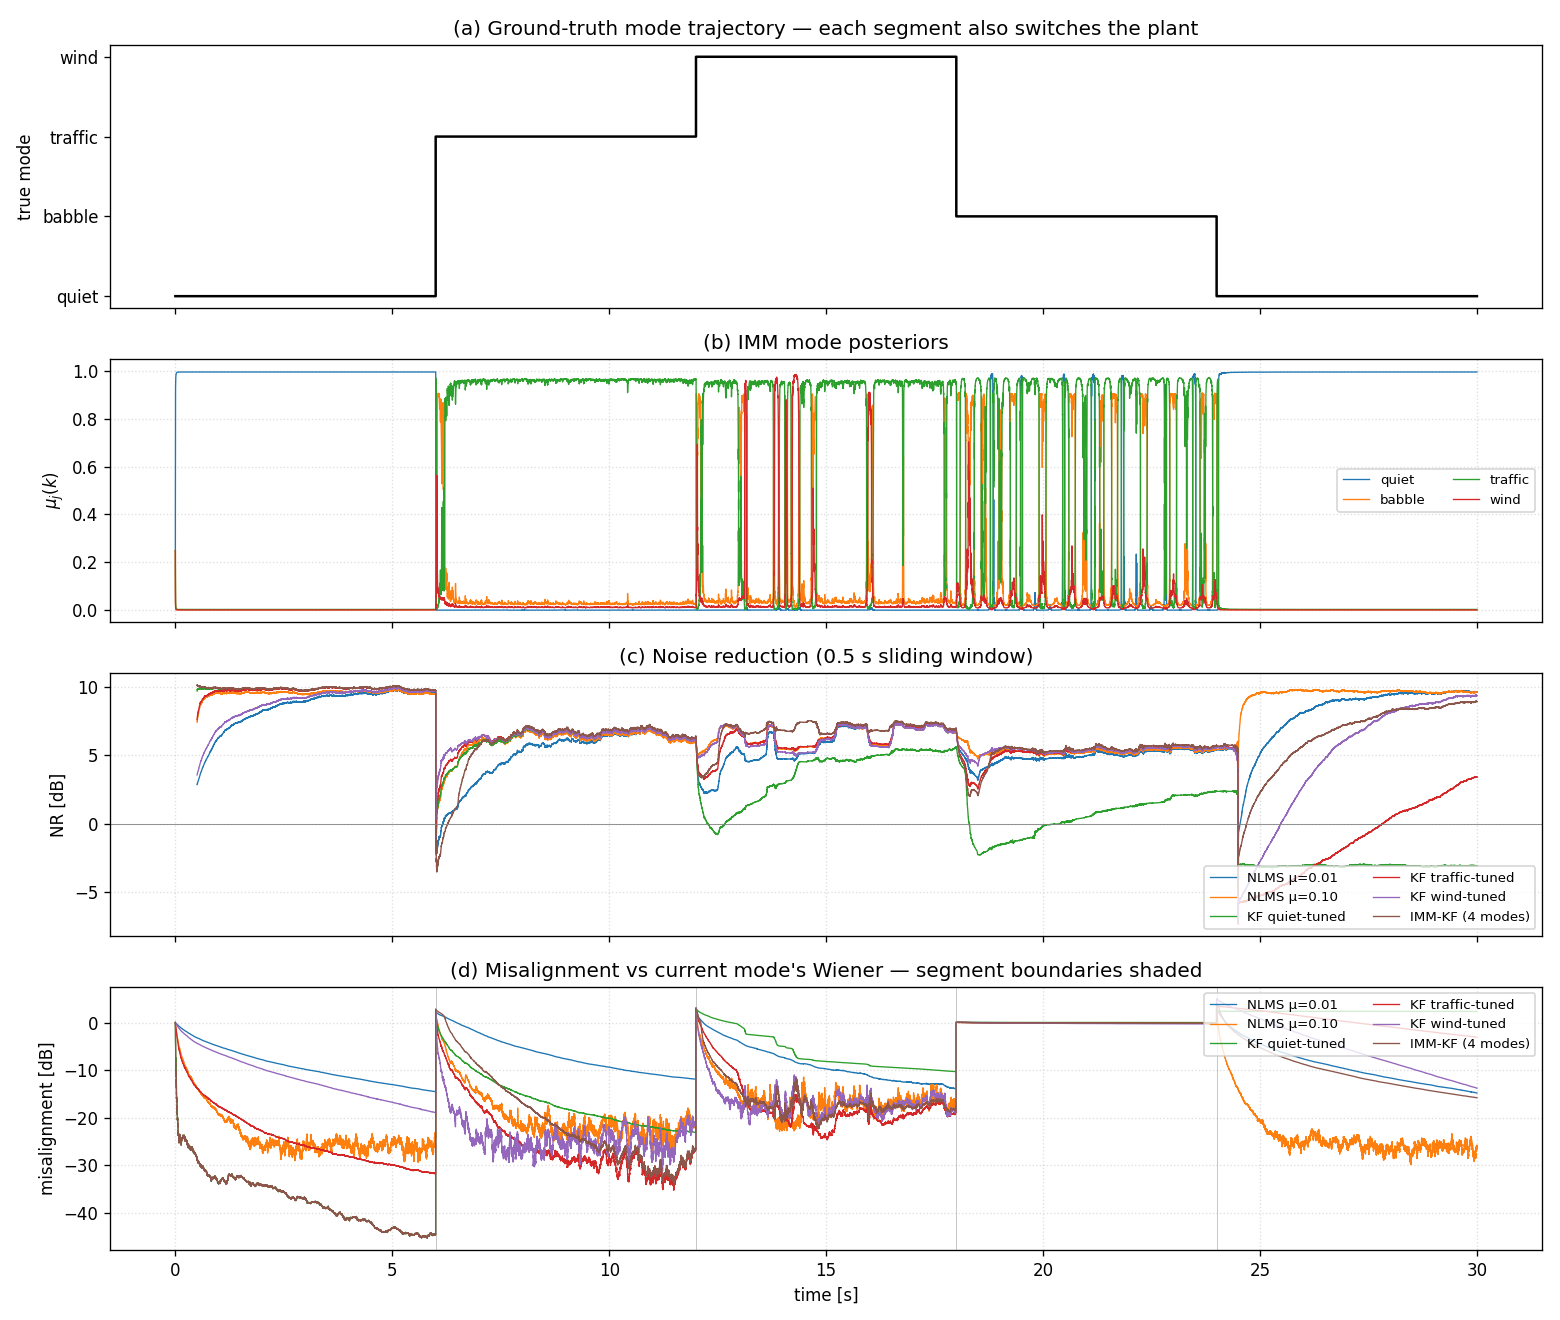
\includegraphics[width=\columnwidth]{figures/05_dynamic_imm.png}
\caption{Dynamic scenario in which the plant switches with the mode. From the top:
the true trajectory of the mode; the posteriors of the modes $\mu_j(k)$; the NR over
a sliding window for all methods; the misalignment against the Wiener reference of
the current mode. Vertical lines mark the boundaries of the segments, where the
plant changes.}
\label{fig:dynamic}
\end{figure}

\subsection{Statistical evaluation by Monte Carlo}
Table~\ref{tab:mc} and Fig.~\ref{fig:mc} summarize an evaluation by Monte Carlo over
fifteen folds; each run draws independent random paths and noise for every mode.

\begin{table}[t]
\caption{Summary of the Monte Carlo evaluation ($N=15$ runs, dynamic scenario with a plant that switches with the mode).}
\label{tab:mc}
\centering
\renewcommand{\arraystretch}{1.15}
\begin{tabular}{@{}lcc@{}}
\toprule
Method               & Mean NR [dB]   & Std [dB] \\
\midrule
\textbf{IMM-KF}      & \textbf{+16.06}& \textbf{1.77} \\
NLMS $\mu=0.10$      & +6.51          & 1.95 \\
KF (wind)            & +5.98          & 2.14 \\
NLMS $\mu=0.01$      & +4.92          & 1.42 \\
KF (traffic)         & +3.68          & 1.11 \\
KF (quiet)           & +2.63          & 0.86 \\
\midrule
\multicolumn{3}{c}{Accuracy of mode tracking for the IMM: $17.9\%\pm5.4\%$} \\
\bottomrule
\end{tabular}
\end{table}

\begin{figure}[t]
\centering
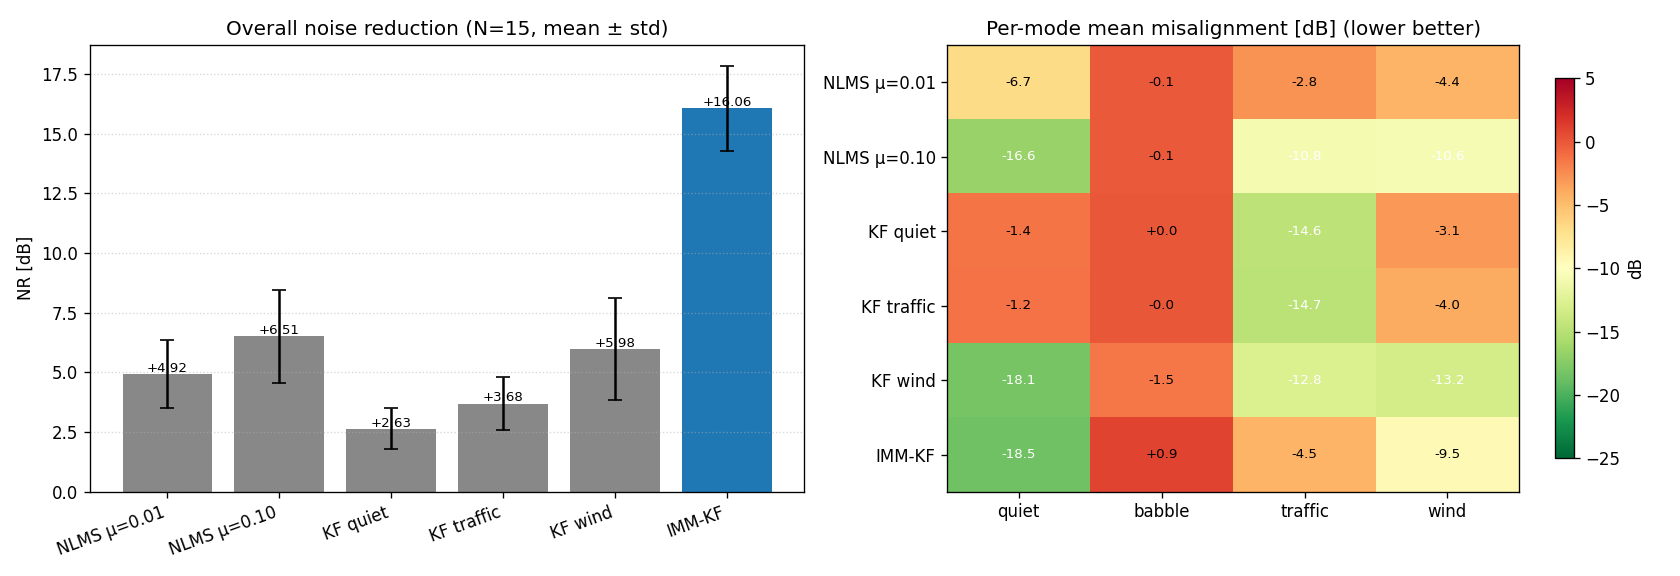
\includegraphics[width=\columnwidth]{figures/06_monte_carlo.png}
\caption{Monte Carlo over $N=15$ runs. Left: the overall NR with error bars of one
standard deviation. Right: a heatmap of the mean misalignment for each mode (lower
is better).}
\label{fig:mc}
\end{figure}

The IMM-KF reaches \SI{+16.06}{\decibel}, more than $2.4$ times the best single
baseline, with the lowest standard deviation among the strong performers. The Kalman
filter tuned for quiet, which wins the static benchmark, is the worst on the dynamic
scenario at \SI{+2.63}{\decibel}, more than fifteen standard deviations below the
IMM-KF, a clear refutation of the implicit assumption that one fixed $Q$ suffices.

\subsection{Mixing is the engine, not classification}
A striking feature of Table~\ref{tab:mc} is that the IMM-KF wins decisively on NR
while its accuracy of tracking the mode is only $17.9\%$, below the value of $25\%$
that a random guess would give over four modes. The two facts are reconciled by a
look at the mixing step. The posterior collapses onto the mode with the lowest
variance of innovation, namely traffic, so the IMM is a poor classifier of the
environment. Yet at every sample the mixing step reseeds the states of all four
modes from one another, and the agile babble filter ($\sigma_q^2=10^{-2}$) supplies
a component that tracks quickly and that the combination inherits. When we ablate the
mixing step, by setting $\Pi=\mathbf{I}$ so that the four filters never exchange
information, the NR collapses from \SI{+16.6}{\decibel} to \SI{+1.5}{\decibel}. The
conclusion is that the accuracy of mode tracking is not the indicator that matters
for this system. The IMM acts as a bank of adaptation speeds that reseeds itself,
and the mixture realizes an effective $(Q,R)$ that varies continuously; the metric
that matters is the NR together with its variance from run to run.

\subsection{Consistency of the filter}
The tests of the normalized estimation error squared (NEES) and of the normalized
innovation squared (NIS) indicate an apparent overconfidence in the covariance of
the combination. This is an artefact of the synthetic scenario, which switches the
acoustic plant at once and injects a brief transient after the switch. Restricting
the statistic to windows in steady state, at least \SI{1}{\second} after each switch,
returns it close to its band of $\chi^2$, and gradual crossfades of equal power,
as used by the listening bench, reduce the transient further.

\subsection{Perceptual evaluation}
Fig.~\ref{fig:thirdoct} reports the noise reduction in separate bands. The active
controllers concentrate their reduction below the crossover at
\SI{1.2}{\kilo\hertz}, exactly the band where real active ANC operates, while the
passive seal handles the high frequencies. The character that results, of a rumble
that is gone while the voices remain, matches the everyday experience of ANC.
Fig.~\ref{fig:spectro} shows the spectrograms from the virtual headphone.
Table~\ref{tab:perc} collects the perceptual measures under a mix of music and
noise. The IMM-KF removes the most noise, with a loudness drop of
\SI{+13.9}{\decibel} on the A scale and the highest recovery of the music by SI-SDR,
yet it also carries the highest index of musical noise, a concrete instance of the
tension between the metric and perception that the NR alone hides. NLMS, by contrast,
is only modestly quieter yet sounds smoother. Making this trade-off both audible,
through the rendering at a shared gain, and measurable, through the index of musical
noise, is, we argue, as important a contribution as the result in decibels.

\begin{table}[t]
\caption{Perceptual measures on the mix of music and noise (one representative run).}
\label{tab:perc}
\centering
\renewcommand{\arraystretch}{1.15}
\begin{tabular}{@{}lcccc@{}}
\toprule
Method & Ctrl.\ NR & dBA drop & SI-SDR & Musical noise \\
       & [dB]      & [dB(A)]  & [dB]   & (lower is natural) \\
\midrule
\textbf{IMM-KF} & \textbf{+16.3} & \textbf{+13.9} & \textbf{+16.3} & $-0.01$ \\
NLMS $\mu=0.10$ & +4.5           & +4.7           & +4.6           & $\mathbf{-0.52}$ \\
KF (wind)       & +4.5           & +5.1           & +4.6           & $-0.42$ \\
\bottomrule
\end{tabular}
\end{table}

\begin{figure}[t]
\centering
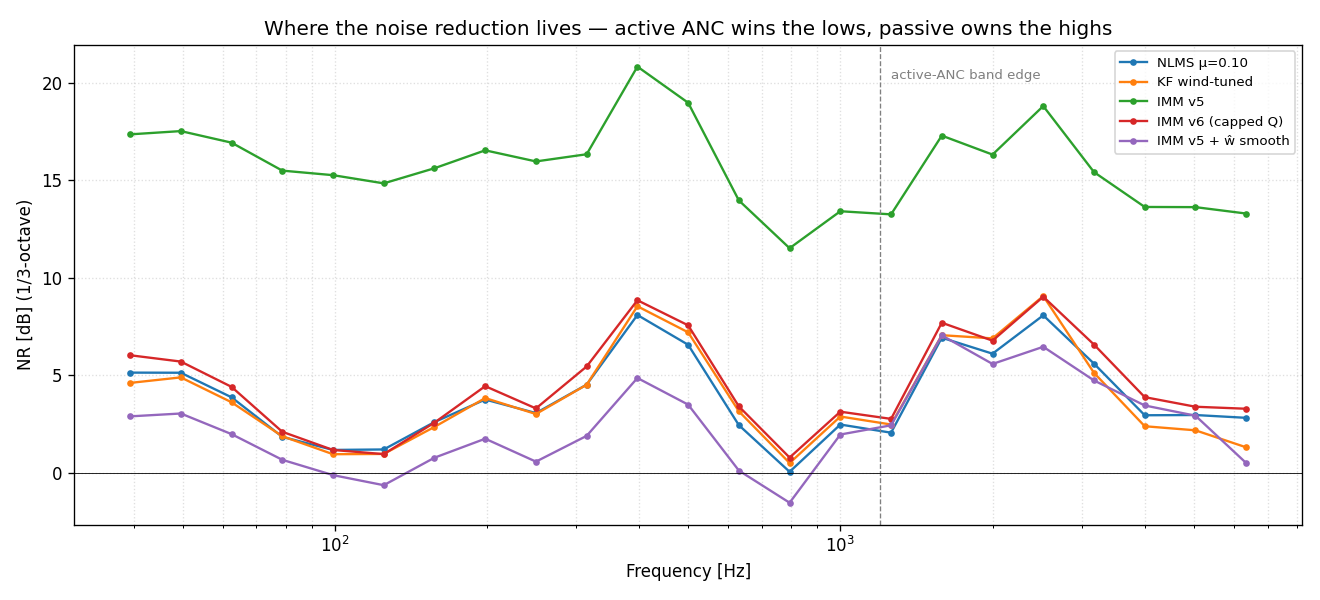
\includegraphics[width=\columnwidth]{figures/20_third_octave_nr.png}
\caption{Noise reduction in third octave bands. The active controllers win the low
band; above the crossover at \SI{1.2}{\kilo\hertz}, shown dashed, the passive seal
dominates.}
\label{fig:thirdoct}
\end{figure}

\begin{figure}[t]
\centering
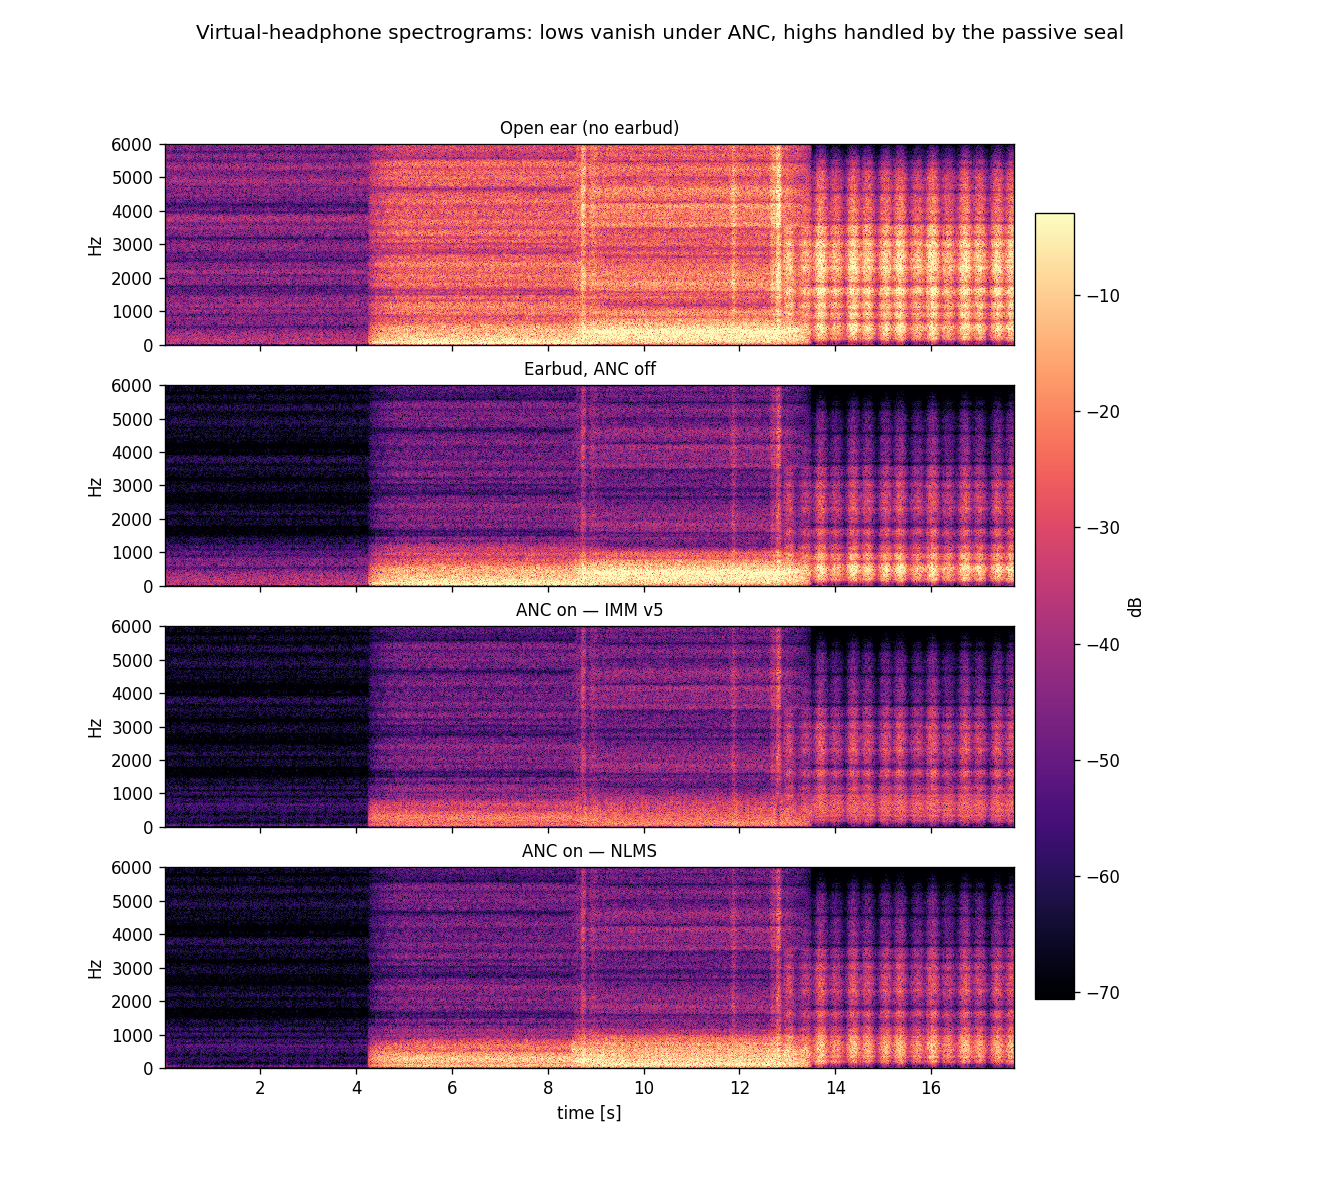
\includegraphics[width=\columnwidth]{figures/20_spectrograms.png}
\caption{Spectrograms from the virtual headphone. The energy at low frequencies
vanishes under the ANC, while the passive seal handles the high frequencies.}
\label{fig:spectro}
\end{figure}

\section{Implementation, Timing, and Demonstration}

\subsection{The C port and its timing}
At \SI{16}{\kilo\hertz}, each sample must be processed within
\SI{62.5}{\micro\second}. We provide a C port of NLMS, of the single mode KF, and of
the IMM-KF that matches the NumPy reference to machine precision. On a desktop CPU at
$L=64$, the step of the IMM-KF costs \SI{56}{\micro\second} in portable scalar C
against \SI{495}{\micro\second} in Python, a speedup of $8.8$ times that places the
controller inside the timing budget (Fig.~\ref{fig:cport}). A build on OpenBLAS is
slower, at \SI{77}{\micro\second}, at this small $L$ because the overhead of the BLAS
calls exceeds their benefit. Deployment in real time on a hearable DSP, with a budget
of 300 to \SI{700}{MIPS} at \SI{100}{\milli\watt}, is therefore a matter of
engineering in fixed point, not of feasibility of the algorithm.

\begin{figure}[t]
\centering
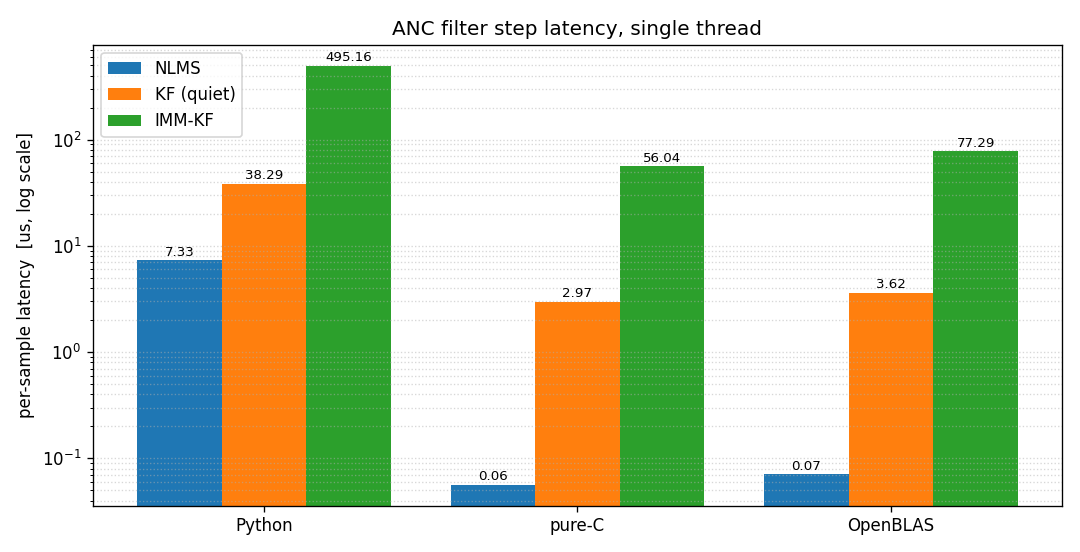
\includegraphics[width=\columnwidth]{figures/08_c_port_speed.png}
\caption{Latency per sample of the C port against the NumPy reference. The dashed
line marks the budget of \SI{62.5}{\micro\second} at \SI{16}{\kilo\hertz}.}
\label{fig:cport}
\end{figure}

\subsection{Interactive demonstration}
One unified application with several pages, built with Streamlit, makes every choice
something the user can experience. A page named Performance Lab runs the controller
live and reports the NR, the tracking of the mode, the factor relative to real time,
the NR by frequency, and the perceptual measures. A page named Music and Feel renders
the ladder of loudness through the virtual headphone, together with a comparison of
the music with and without the ANC at a shared gain, so that the listener experiences
both the cancellation and any artefacts. The application reuses the same core of
orchestration as the batch pipeline, so all the audio is identical to the results we
report. The full implementation, the test bench, and the interactive application are
openly available.\footnote{\url{https://github.com/yesinali/IMM-KF-adaptive-ANC-for-hearables}}

\section{Discussion and Limitations}

The advantage of the IMM-KF on the pair of metrics, mean and variance, is consistent
with the argument that a bank of adaptation speeds that reseeds itself dominates a
fixed tuning in environments that are nonstationary. Three honest limitations remain.
First, the bank is a poor classifier in the explicit sense: because the modes differ
mainly in $(Q,R)$ and not in the observation model, the likelihoods of the
innovation at the sample rate cannot separate them, and the system should be
understood as an adaptive blender rather than a detector of the environment. Second,
the synthetic babble generator has a modulated amplitude and so violates the
assumption of a stationary Wiener solution, so the misalignment for that mode is not
informative for any method. Third, the model of the plant is a random FIR with an
envelope that decays exponentially, a reasonable analytical proxy that does not
capture real resonances or behaviour that is not minimum phase; measurements on a
real head would tighten the conclusions. Finally, the noise and the program material
are synthetic or supplied by the user; the pipeline exposes an interface that lets
the recordings of the DEMAND and ESC-50 datasets replace the generators without any
change to the code, a path we verified with clips from both datasets.

\section{Conclusion}

We formulated, calibrated, and evaluated an Interacting Multiple Model Kalman filter
for the adaptive controller of a feedforward hearable ANC system. The linear state
space form of the model on the FIR coefficients removes any need for the EKF or the
UKF. Across fifteen Monte Carlo runs on a dynamic scenario in which the plant
switches with the mode, the IMM-KF reached the highest mean noise reduction,
\SI{+16.06}{\decibel} with a standard deviation of \SI{1.77}{\decibel}, against
\SI{+6.51}{\decibel} for NLMS and \SI{+2.63}{\decibel} for the quiet Kalman filter
that wins the static benchmark, and an ablation attributed this gain to the mixing
step of the IMM and not to classification of the mode. Beyond decibels, a virtual
headphone test bench and a set of perceptual measures exposed a tension between the
metric and perception, and a C port that matches the reference to machine precision
met the timing budget at \SI{56}{\micro\second} per sample. Future work includes the
estimation of the residual variance online for an adaptive $R$ in each mode, a
hierarchy of IMM that recovers the ability to classify, models of the plant from a
real head, and an integration with estimators of the Kalman gain that are learned,
such as KalmanNet.

\section*{Acknowledgment}
Prepared for EE4084 (Kalman and Bayesian Filters), Department of Electrical and
Electronics Engineering, Marmara University, instructed by Prof.\ Dr.\ Engin
Masazade.

During the preparation of this manuscript, the authors used Claude for editing
and grammatical enhancement to improve the readability of text written by the
authors. Claude was also used as a programming assistant during the
implementation of the interactive web-based demonstration interface. The
concepts, system requirements, the IMM-KF formulation and its calibration
methodology, the virtual-headphone evaluation approach, and the experimental
procedures were developed and specified by the authors. All code and textual
modifications produced with AI assistance were reviewed, tested, and revised by
the authors, who assume full responsibility for the final manuscript and
software.

\bibliographystyle{IEEEtran}
\bibliography{refs}

\end{document}
